\section{Reconstruction using SPINE}

When working with LArTPC detectors, fundamentally, all it returns is a series of voltages that have been read out to the  readout chips.
To get to a physics object from just a number of  voltages, a lot of work has to be done.
This process of converting from raw hits
\footnote{The individual voltages from a channell}
to physics objects is called reconstruction.

\begin{figure}[H]
  % 
  \centering
  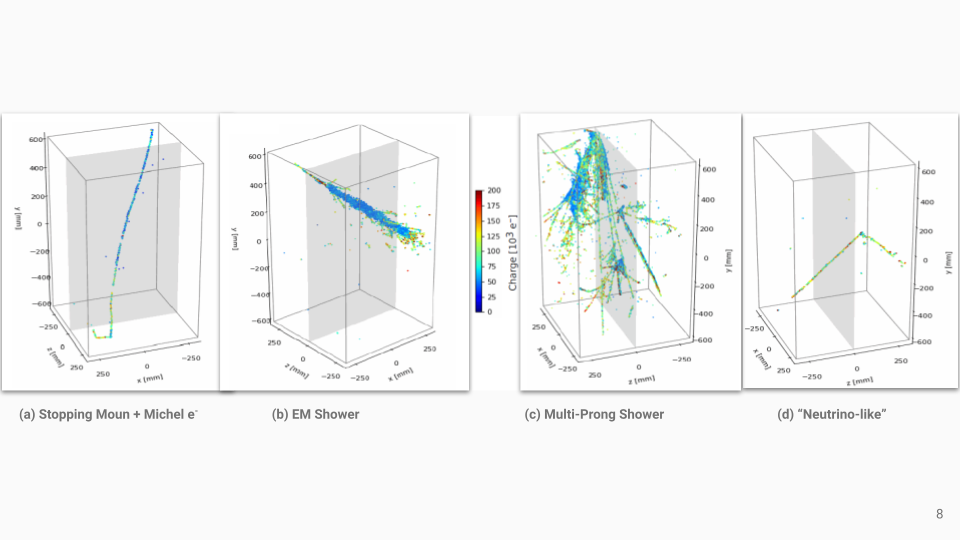
\includegraphics[width=120mm]{figures/mod0Events.png}
  \caption{Some reconstructed events from the module-0 prototype for the DUNE Near Detector}
  \label{mod0Event}
\end{figure}

There are a number of algorithims to do reconstruction of events, oftentimes with their own idiosyncracies, advantages and disadvantages.
The SPINE package is one that uses machine learning to perform this reconstruction.

\subsection{The SPINE Reconstruction Pipeline}